\documentclass{standalone}
\usepackage{standalone}

\begin{document}
\section{Linear Regression}
Linear regression is a linear approach to compute the relationship between the dependent variable and the independent variables. Linear regression is often used in predictive analysis. In linear regression, a straight line is drawn which follows the below equation  and known as hypothesis function.
\begin{center}
	\makebox[\textwidth]{h {\textsubscript{\theta}} {(x)} =  \theta ^{T}x}
	\caption{Equation for Linear regression.}
\end{center}
\\
Here,\\
$ \X\theta $ = Denotes co-efficient matrix\\
X = Denotes the matrix of independent variables}\\
h\textsubscript{ $ \theta $}{(x)} = Denotes a hypothesis function.\\

\begin{figure}[h]
				\centering
				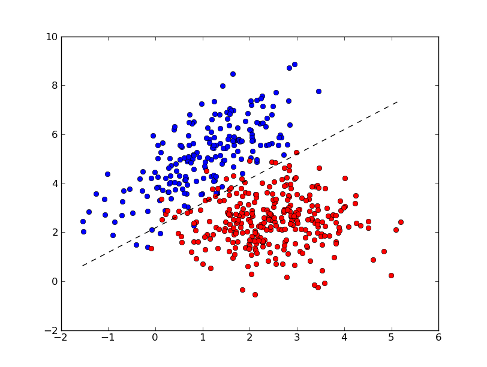
\includegraphics[scale=1.0]{./img/lir}
				\caption{Basic Linear Regression} \label{fig:mapComp}
\end{figure}


The coefficients $\theta$ are derived using the cost function, J($\theta$) which is shown in following equation. When the cost function is minimized the values of the coefficients are considered derived.\\
\begin{center}
	\makebox J($\theta$) = $\frac{1}{2m} \sum_{i=1}^{m}(h\textsubscript{$\theta$}(x\textsubscript{i})-y\textsubscript{i})^{2}  $ \\
\end{center}
\\
Here, \\
m is the number of features\\
Y\textsubscript{i} is an element of output set Y = {y\textsubscript{1}, y\textsubscript{2}, y\textsubscript{3}, ... , y\textsubscript{n}} of the training data set.\\

\end{document}